\chapter{Kinematics}

\section{Rectilinear Motion}

\subsection{Time Derivatives of Position}

\begin{definition}
    The \vocab{distance} ($d$) travelled by a body is the length of the path it has taken.
\end{definition}

Distance is a scalar quantity. Its SI unit is metre (m).

\begin{definition}
    \vocab{Displacement} ($s$, $x$) is the straight-line distance and the direction from a fixed point.
\end{definition}

Displacement is a vector quantity. Its SI unit is metre (m).

\begin{definition}
    \vocab{Speed} ($v$) is the distance travelled per unit time.
\end{definition}

Speed is a scalar quantity. Its SI unit is metre per second (m s$^{-1}$).

\begin{definition}
    \vocab{Velocity} ($v$) is the rate of change of displacement. \[v = \der{x}{t}.\]
\end{definition}

Velocity is a vector quantity. Its SI unit is metre per second (m s$^{-1}$).

\begin{definition}
    \vocab{Acceleration} ($a$) is the rate of change of velocity. \[a = \der{v}{t}.\]
\end{definition}

Acceleration is a vector quantity. Its SI unit is metre per second square (m s$^{-2}$).

\subsection{Graphical Methods}

Given a displacement-time ($s$-$t$) graph, the velocity $v$ is given by the gradient of the graph.

Given a velocity-time ($v$-$t$) graph,
\begin{itemize}
    \item the change in displacement $\D s$ in any time interval $\D t$ is given by the corresponding signed area under the graph; and
    \item the acceleration is given by the gradient of the graph.
\end{itemize}

\subsection{Equations of Motion}

\begin{theorem}[Equations of Motion]
    Consider a body moving with uniform acceleration $a$ in a straight line. If its initial velocity is $u$, and its final velocity at time $t$ is $v$, then
    \begin{tasks}(3)
        \task $v = u + at$,
        \task $\displaystyle s = \frac{u+v}{2} t$,
        \task $\displaystyle s = ut + \frac12 at^2$,
        \task $\displaystyle s = vt - \frac12 at^2$,
        \task $v^2 = u^2 + 2as$.
    \end{tasks}
\end{theorem}

\subsection{Free-Fall}

\begin{definition}
    \vocab{Free-falling} refers to motion under the influence of a uniform gravitational field without air resistance.
\end{definition}

A free-falling body undergoes uniformly accelerated motion in the vertical direction. Using the equations of motion, we see that (taking the upward direction as positive): \[s = ut - \frac12 gt^2 \quad \tand \quad v = gt,\] hence the body follows a parabolic trajectory, and the speed of the body will increase uniformly as it falls.

For a body projected upward, the motion has a \emph{speed symmetry}, i.e. the speed $v$ during the upward motion is equal to the speed $v$ at the same point during the downward motion. Accordingly, there would also be a \emph{time symmetry}, i.e. the time $\D t$ for the body to reach maximum height from any point is equal to the time $\D t$ for it to return to the same point.

\begin{definition}
    \vocab{Air resistance} ($R$) is the resistive force acting on a body moving through air.
\end{definition}

The direction of air resistance is always opposite that of motion. At low velocities, $R \propto v$. At high velocities, $R \propto v^2$.

If the body remains long enough in the air, eventually $R \to W$, and it will no longer accelerate. The body has reached \vocab{terminal velocity}.

\begin{figure}[H]
    \centering
    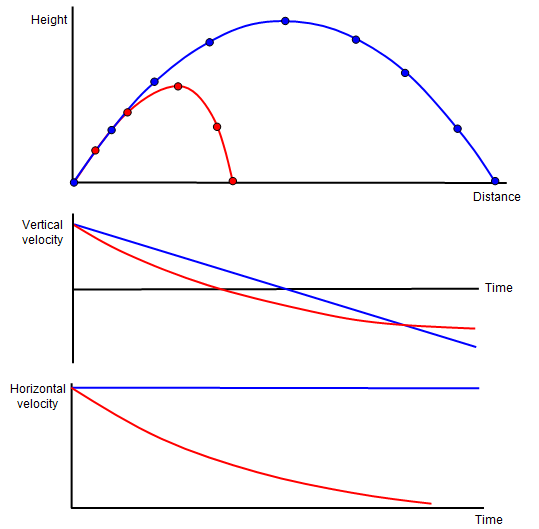
\includegraphics[scale=0.5]{media/Free Fall.png}
    \caption{The $s$-$t$ and $v$-$t$ graphs for {\color{blue} negligible} and {\color{red}non-negligible} air resistance.\protect\footnotemark}
\end{figure}
\footnotetext{Source: \url{https://www.schoolphysics.co.uk/age16-19/Mechanics/Kinematics/text/Projectiles_and_air_resistance/index.html}}

\section{Projectile Motion}

\begin{definition}
    \vocab{Projectile motion} refers to the motion of a body in which there is a uniform velocity in one direction and a uniform acceleration in a perpendicular direction.
\end{definition}

Consider an idealized model, where the projectile is a particle with acceleration (due to gravity) that is constant in both magnitude and direction. Note that the plane of motion is two-dimensional since the acceleration due to the gravity is purely vertical (the projectile cannot move sideways). We represent this plane of motion with the $xy$-plane. The trajectory of the object depends only on the initial velocity $u$ and the downward acceleration due to gravity $g$.

By treating the $x$- and $y$-coordinates separately, we can easily analyse projectile motion. With initial speed $u$ and projection angle $\a$, we obtain the following formulae:
\begin{itemize}
    \item In the \emph{horizontal direction}, there is no resultant force, so $a_x = 0$. By the equations of motion, we get
    \begin{align*}
        a_x &= 0,\\
        v_x &= u_x\\
        &= u \cos \a,\\
        s_x &= u_x t\\
        &= \bp{u \cos \a} t.
    \end{align*}
    \item In the \emph{vertical direction}, there is a constant acceleration of $-g$. Taking the upwards direction as positive, we get
    \begin{align*}
        a_y &= -g, \\
        v_y &= u_y - gt \\
        &= u \sin \a - gt, \\
        s_y &= u_y t - \frac12 gt^2\\
        &= \bp{u \sin \a} t - \frac12 gt^2.
    \end{align*}
\end{itemize}

The magnitude $v$ and direction $\t$ of the velocity of the particle at any instant can be calculated using \[v = \sqrt{v_x^2 + v_y^2} \quad \tand \quad \t = \arctan \frac{v_y}{v_x}.\]

\begin{proposition}
    The time to reach the maximum height is $u \sin \a / g$.
\end{proposition}
\begin{proof}
    At maximum height, $v_y = 0$. Thus, \[u\sin \a - gt = 0 \implies t = \frac{u \sin \a}{g}.\]
\end{proof}
Using time symmetry, we easily obtain the total flight time of the body.
\begin{corollary}
    The total time of flight is $2u\sin \a / g$.
\end{corollary}

\begin{proposition}
    The maximum height attained by the particle is $u^2 \sin^2 \a / 2g$.
\end{proposition}
\begin{proof}
    We know the body is highest when $t = u \sin \a / g$. Substituting this into the equation for $s_y$, we get \[s_y = \bp{u \sin \a}\bp{\frac{u \sin \a}{g}} - \frac12 g \bp{\frac{u \sin \a}{g}}^2 = \frac{u^2 \sin^2 \a}{2g}.\]
\end{proof}

\begin{proposition}
    The range (maximum horizontal distance covered by the trajectory) is $u^2/g$.
\end{proposition}
\begin{proof}
    We know that it takes $t = 2u\sin \a/g$ for the object to land. Substituting this into the equation for $s_x$, \[s_x = \bp{u \cos \a} \bp{\frac{2u \sin \a}{g}} = \frac{u^2 \sin 2\a}{g}.\] Clearly, $s_x$ is maximized when $\sin 2\a = 1$ (i.e. $\a = \pi/4$), whence the range is $u^2/g$.
\end{proof}